% !TEXroot=main.tex
\section{Lokalisierung}
{	
	\subsection{Positionierung auf einer Karte}
	{
		
	Um den Roboter Korrekt auf der Karte zu Lokalisieren, wird die Monte-Carlo-Lokalisation verwendet. Als Messpunkte dienen die Daten des LiDAR-Sensors. In der beigefügten Abbildung, wird das vergleichen von Sensordaten und Karte deutlich.
		\begin{figure}[H]
			\centering
			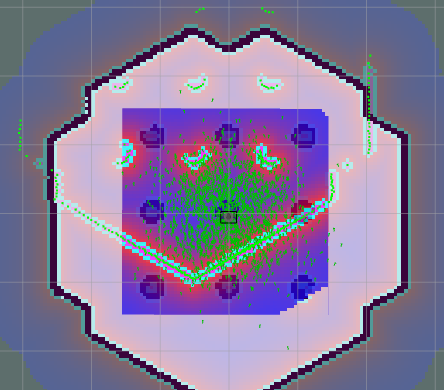
\includegraphics[height=5cm]{Bilder/costmap_monte_carlo_example.png}
			\caption{Costmap mit Sensordaten} 
			\label{pic:coastmontecarlo}
		\end{figure}
		In der Abbildung wird deutlich, dass der Roboter auf der gegebenen Karte (Hintergrund) mittig platziert wird. Gleichzeitig misst der LiDAR-Sensor auch Hindernisse, welche wiederum eine neue Karte der Umgebung bilden. Diese Hindernisse sind hell im Vordergrund zu sehen. Man erkennt, dass diese nicht übereinander liegen und der Roboter deshalb noch nicht korrekt positioniert ist. In Wirklichkeit werden Daten aus der unteren linken Ecke der Karte gemessen. Dadurch werden Positionen in dieser Umgebung sehr wahrscheinlich. Damit der Roboter bei vielen ähnlichen Stellen, was hier nicht der Fall ist, trotzdem korrekt positioniert ist, wird der Roboter zwischen verschiedenen LiDAR-Messungen bewegt. Während der Bewegungen wird errechnet, wo der Roboter sich, ausgehend von den Ursprünglichen Vermutungen der Position, befindet. Stimmen auch die neuen Messungen mit der Karte überein, so wird eine Position immer wahrscheinlich, bis der Roboter schlussendlich, sicher positioniert werden kann, da Sensordaten und Karte übereinstimmen. im Falle anderer Roboter können neben LiDAR-Sensoren auch andere Sensordaten verwendet werden.
	}
}